\documentclass[border=2pt]{standalone}
\usepackage{tikz}
\usetikzlibrary{arrows.meta,calc,shapes.symbols}
\begin{document}
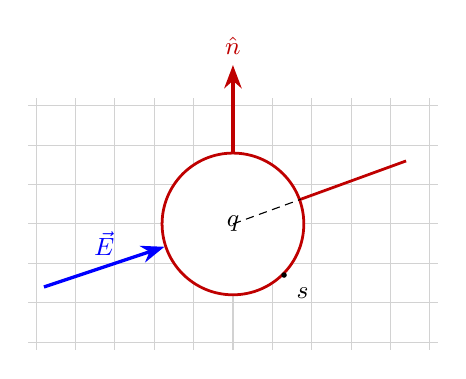
\begin{tikzpicture}[>=Stealth,every node/.style={font=\small},
  vector/.style={->,very thick}]
  \draw[gray!35] (-2.6,-1.6) grid[step=.5] (2.6,1.6);
  \node[magnifying glass,draw=red!75!black,fill=white,line width=1pt,
    minimum size=18mm,magnifying glass handle angle=20,
    magnifying glass handle aspect=1.6] (probe) {$q$};
  \draw[vector,blue] (-2.4,-.8) -- (probe)
    node[midway,above] {$\vec E$};
  \draw[vector,red!75!black] (probe.north) -- ++(0,1.1)
    node[above] {$\hat n$};
  \draw[densely dashed] (probe.center) -- (probe.20);
  \fill (probe.south east) circle (1pt) node[below right=1pt] {$s$};
\end{tikzpicture}
\end{document}
